% ==============================================================================
\section{Módulo de navegación}
\label{sec:dev_nav}
% ==============================================================================

\subsection{Descripción}

El módulo de navegación decide, paso a paso, qué debe hacer el usuario para llegar a
su destino: avanzar, girar a la izquierda, girar a la derecha o detenerse. La decisión
la toma un agente de aprendizaje por refuerzo profundo entrenado en simulación con el
algoritmo PPO, tal como se planteó en TT1. Alrededor del agente se construyeron tres
piezas que no estaban en el diseño original: un ejecutor que administra la sesión y
traduce las acciones en frases, una capa de seguridad determinística que puede
anular al agente y un planificador que anticipa la ruta completa para mostrarla en la
interfaz. El módulo cubre los requerimientos RF-18 a RF-21 y RF-23.

Los destinos ya no provienen de un servicio de cartografía. Cuando el usuario pide
``llévame a la salida'', el ejecutor busca entre los \emph{landmarks} del SLAM el más
cercano con la etiqueta correspondiente (puerta, en este caso) y lo toma como meta.
También se acepta un punto explícito del mapa, lo cual se usa durante las pruebas.

\subsection{Entorno de entrenamiento}

El agente se entrena en un entorno propio construido con Gymnasium
(\texttt{navigation/nav\_env.py}). Cada episodio genera un mundo nuevo de uno de tres
tipos:

\begin{itemize}
    \item \textbf{Cuarto} (40\,\% de los episodios): un rectángulo de 4 a 9~m por 3.5 a
    7~m con entre dos y cinco muebles, hasta un peligro de piso y hasta una persona en
    movimiento.
    \item \textbf{Dos cuartos con puerta} (35\,\%): dos cuartos separados por una pared
    con un vano de 0.9 a 1.3~m. El inicio está en un cuarto y la meta en el otro, de
    modo que el agente debe encontrar la puerta.
    \item \textbf{Exterior} (25\,\%): un área abierta de 10 a 18~m por 8 a 14~m con
    postes dispersos, de una a tres coladeras y hasta dos personas.
\end{itemize}

Las personas se desplazan entre 5 y 12~cm por paso, rebotan en los límites y de vez
en cuando cambian de dirección. Los peligros de piso no bloquean los rayos, igual que
en el sistema real, donde un hoyo no produce eco ni detiene la vista: el agente solo
los conoce por la distancia por sector que le llega en la observación. Además de los
mundos generados, en aproximadamente la mitad de los episodios se usa uno de los 19
mapas reales obtenidos de video (Sección~\ref{sec:dev_mapeo}). Para ello, las celdas
ocupadas se convierten en obstáculos circulares, la capa de peligros en coladeras, y
el inicio y la meta se eligen dentro de la misma zona libre conexa, con al menos
30~cm de holgura respecto a cualquier obstáculo.

\subsection{Acciones, observación y recompensa}

Las acciones son las cuatro definidas en TT1: avanzar 0.30~m, girar $20^\circ$ a la
izquierda, girar $20^\circ$ a la derecha y detenerse.

La observación es donde más se apartó la implementación del diseño original. El
vector de ocho valores planteado en TT1 ($d_{\text{front}}$, $d_{\text{left}}$,
$d_{\text{right}}$, $\phi_{\text{goal}}$, $d_{\text{goal}}$ y los tres riesgos) se
implementó y se comparó contra una observación extendida de 24 valores, descrita en la
Tabla~\ref{tab:nav_obs}. Con el mismo presupuesto de entrenamiento, la observación
extendida obtuvo 85.8\,\% de episodios exitosos contra 44.2\,\% de la original
(Figura~\ref{fig:nav_comparacion}). La diferencia se concentra en los mundos con
puerta: con solo tres distancias por sector, el agente no ``ve'' el hueco de la puerta
y fracasa en nueve de cada diez intentos.

\begin{table}[H]
\centering
\caption{Componentes de la observación extendida (24 valores normalizados)}
\label{tab:nav_obs}
\renewcommand{\arraystretch}{1.25}
\begin{tabular}{|c|p{11.8cm}|}
\hline
\textbf{Valores} & \textbf{Contenido} \\
\hline
11 & Distancia libre en 11 direcciones entre $-100^\circ$ y $+100^\circ$, divididas
entre el alcance máximo de 4~m. \\
\hline
3 & Distancia al peligro de piso más cercano en cada sector (frente, izquierda,
derecha), divididas entre 3~m. \\
\hline
3 & Nivel de riesgo por sector, dividido entre 3. \\
\hline
3 & Dirección a la meta como $\sin\phi_{\text{goal}}$ y $\cos\phi_{\text{goal}}$, y
distancia a la meta acotada a 10~m. \\
\hline
4 & Acción anterior en codificación \emph{one-hot}. \\
\hline
\end{tabular}
\end{table}

\begin{figure}[H]
    \centering
    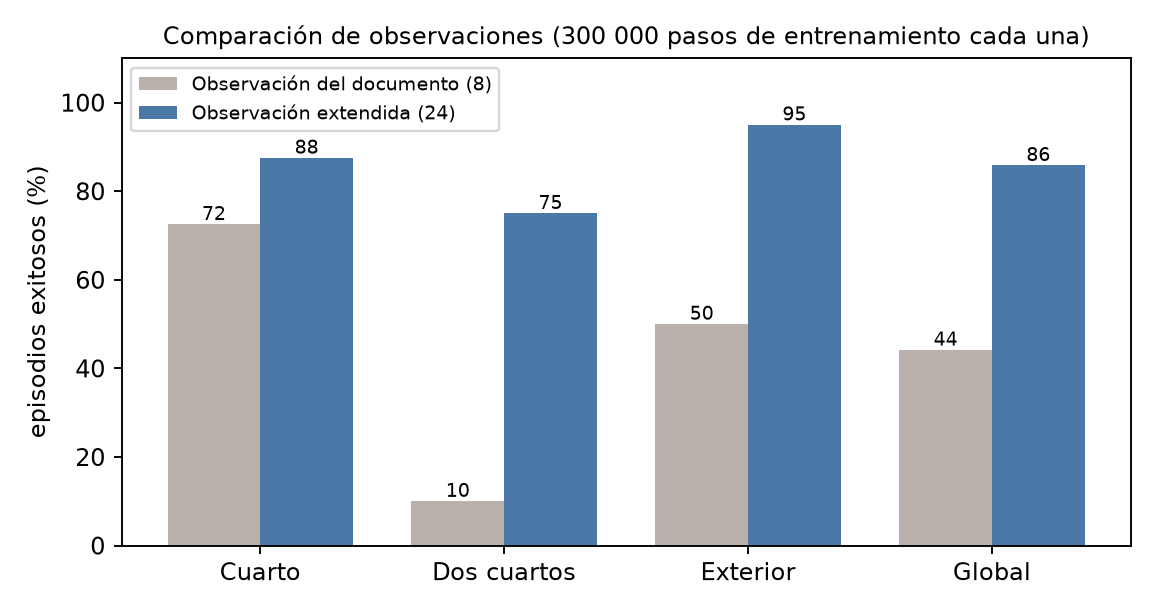
\includegraphics[width=0.78\textwidth]{Capturas_TT2/nav/nav_comparacion_obs.png}
    \caption{Porcentaje de episodios exitosos con la observación del documento y con la
    observación extendida, tras 300\,000 pasos de entrenamiento cada una.}
    \label{fig:nav_comparacion}
\end{figure}

La recompensa sigue la estructura de TT1, pero con escalas ajustadas. Con los
coeficientes originales, la penalización por riesgo pesaba tanto que el agente
aprendía a quedarse quieto. La versión final es:

\[
r_t = -0.1 + 4\,(d_{t-1} - d_t) - 0.15\, r_{\text{front}}
      + \begin{cases}
      +100 & \text{si llega a menos de 0.45~m de la meta} \\
      -100 & \text{si choca o cae en un peligro de piso} \\
      +0.5 & \text{si se detiene con una persona a menos de 1.2~m enfrente} \\
      -0.3 & \text{si se detiene sin motivo}
      \end{cases}
\]

donde $d_t$ es la distancia a la meta. El término de detenerse se agregó para que la
acción tuviera una función clara: esperar a que una persona termine de cruzar.

Para reducir la diferencia entre la simulación y el sistema real se añadió ruido de
5\,\% a las distancias, de $2^\circ$ al ángulo de la meta y, en el 8\,\% de los rayos
bloqueados, se reporta el alcance máximo como si estuvieran libres. Esta última
perturbación imita lo que ocurre en el mapa real, donde un rayo delgado puede colarse
entre dos celdas de eco separadas (Sección~\ref{sec:dev_ray}) y reportar libre un
frente bloqueado.

\subsection{Entrenamiento}

El agente se entrena con la implementación de PPO de Stable-Baselines3 sobre
PyTorch, con ocho entornos en paralelo. La Tabla~\ref{tab:nav_ppo} resume los
hiperparámetros. El modelo final se entrenó durante 8 millones de pasos. Se exporta en
dos formatos: el archivo completo de Stable-Baselines3, que se usa en la computadora
portátil, y un archivo con solo los pesos de la red del actor, con el que la
Raspberry Pi ejecuta la inferencia en NumPy sin instalar PyTorch. Se verificó que
ambos formatos eligen la misma acción en 500 observaciones aleatorias.

\begin{table}[H]
\centering
\caption{Hiperparámetros de PPO}
\label{tab:nav_ppo}
\renewcommand{\arraystretch}{1.2}
\begin{tabular}{|l|c|}
\hline
\textbf{Parámetro} & \textbf{Valor} \\
\hline
Red del actor y del crítico & dos capas ocultas de 128 neuronas, \emph{tanh} \\
Pasos por actualización (por entorno) & 2048 \\
Tamaño de lote & 512 \\
Factor de descuento $\gamma$ & 0.995 \\
$\lambda$ de GAE & 0.95 \\
Coeficiente de entropía & 0.01 \\
Tasa de aprendizaje & $3 \times 10^{-4}$ \\
Recorte de PPO & 0.2 \\
\hline
\end{tabular}
\end{table}

El modelo pasó por varias iteraciones, evaluadas siempre con el mismo protocolo. Un
primer modelo entrenado solo en mundos generados alcanzó 99.2\,\% de éxito en ellos.
Al incorporar los mapas de video, el peor caso fue un pasillo de oficina muy angosto y
lleno de muebles (v09), donde varios reentrenamientos con más pasos o con otra mezcla
de mapas no lograron superar al modelo vigente. Al revisar ese caso se encontró un
error en el entrenador: en mapas densos el inicio o la meta podían quedar encima de un
obstáculo, lo que producía choques imposibles de evitar. Con el muestreo corregido, el
modelo vigente subió de 82.5 a 85\,\% en ese mapa, y se comprobó que retirar v09 del
entrenamiento empeora el desempeño en pasillos densos, por lo que se conservó en la
mezcla.

\subsection{Ejecución en el dispositivo}

El ejecutor (\texttt{navigation/navigator.py}) es la parte del módulo que corre en el
dispositivo. Mantiene el estado de la sesión (en espera, activa o pausada) con los
mensajes literales del Algoritmo 11 de TT1, recibe los comandos ya interpretados por
el PLN y, en cada ciclo, construye la observación a partir del cuadro de navegación y
del mapa. Para que esa observación se parezca a la del entrenamiento, cada uno de los
11 rayos es el mínimo de un abanico de tres sub-rayos separados $6^\circ$, y las
distancias a los peligros se leen del segundo canal del mapa local.

Sobre la decisión del agente actúan varias reglas fijas:

\begin{itemize}
    \item \textbf{Capa de seguridad.} Si el agente indica avanzar y la distancia libre
    al frente es menor que 0.80~m, ya sea según el mapa o según la visión, la orden se
    reemplaza por un giro. El umbral es el mismo de la alerta crítica, de modo que el
    usuario nunca escucha ``Deténgase'' y ``Avance'' en el mismo instante. El sentido
    del giro se mantiene durante un máximo de ocho giros seguidos (unos $160^\circ$),
    para no alternar izquierda y derecha en una esquina.
    \item \textbf{Ritmo de decisión.} El agente decide una vez por segundo, salvo que
    haya una alerta crítica, en cuyo caso decide de inmediato.
    \item \textbf{Frases.} Cada acción se traduce con las frases exactas de TT1:
    ``Avance N metros'', ``Gire ligeramente a la izquierda'' (giros de hasta
    $45^\circ$), ``Gire a la izquierda N grados'' o ``Deténgase''. La distancia de
    avance se limita a lo que el mapa ve libre y, si la confianza del SLAM baja de
    0.35, a un metro. El aviso ``Está cerca de su destino'' se dice una sola vez por
    destino.
    \item \textbf{Llegada.} La sesión termina cuando la pose queda a menos de 0.6~m de
    la meta o cuando la cámara ve el objeto buscado a menos de 1~m enfrente. La
    segunda condición se agregó porque, sin odometría, la pose deriva y el usuario
    podía quedarse dando vueltas junto al objeto.
    \item \textbf{Bloqueo.} Si en 20~s la distancia a la meta no disminuye al menos
    30~cm, el sistema avisa que no encuentra un paso libre y sugiere pedir otra ruta.
\end{itemize}

El Algoritmo~\ref{alg:dev_nav} resume un ciclo del ejecutor.

\begin{center}
\captionof{algorithm}{Ciclo del ejecutor de navegación}
\label{alg:dev_nav}
\end{center}
\vspace{-1.8cm}
\rule{\textwidth}{0.4pt}
\vspace{-0.9cm}
\begin{algorithmic}[1]

\Statex \textbf{ENTRADA:} cuadro\_nav, mapa, alertas
\Statex \textbf{SALIDA:} lista de mensajes para la salida de voz

\Statex
\If{sesión no está activa}
    \State \Return []
\EndIf
\State d $\gets$ distancia(pose, meta)
\If{d $< 0.6$ m O la cámara ve el objeto meta a menos de 1 m}
    \State sesión $\gets$ ``en\_espera''
    \State \Return [``Ha llegado a su destino.'']
\EndIf
\If{no hay alerta crítica Y pasó menos de 1 s desde la última decisión}
    \State \Return []
\EndIf
\State obs $\gets$ construir\_observación(cuadro\_nav, mapa, meta, acción\_previa)
\State acción $\gets$ política(obs)
\If{acción = avanzar Y distancia\_libre\_al\_frente $< 0.80$ m}
    \State acción $\gets$ giro\_forzado() \Comment{con histéresis de sentido}
\EndIf
\State texto $\gets$ frase(acción, d, $\phi_{\text{goal}}$, distancia\_libre, confianza)
\If{texto es nuevo O pasaron más de 3.5 s desde la última indicación}
    \State agregar texto a mensajes
\EndIf
\If{la distancia a la meta no bajó 0.3 m en 20 s}
    \State agregar aviso de bloqueo a mensajes
\EndIf
\State \Return mensajes

\end{algorithmic}
\vspace{-0.9cm}
\rule{\textwidth}{0.4pt}

\subsection{Planificador de ruta}

El agente decide solo el siguiente paso, lo cual dificulta saber hacia dónde va.
Para visualizarlo, el planificador (\texttt{navigation/route\_planner.py}) simula al
agente sobre el mapa actual desde la pose del usuario, sin moverlo, y registra los
puntos por los que pasaría hasta llegar, quedar atascado o agotar 240 pasos. La ruta
resultante se clasifica como ``llega'', ``bloqueada'' o ``larga'' y se dibuja en la
interfaz. Un plan tarda unos 7~ms; se recalcula cada dos segundos en un hilo aparte, o
de inmediato si llega una alerta crítica. Como las puertas se registran sobre la
pared, cuando la meta cae en una celda ocupada el planificador la traslada a la celda
libre más cercana. La ruta es informativa: la decisión que se le comunica al usuario
sigue siendo la del ejecutor.

\subsection{Resultados}

\textbf{Evaluación del modelo.} El modelo final se evaluó en 880 episodios: 40 en
cada tipo de mundo generado y 40 en cada uno de los 19 mapas reales, con semillas
distintas a las del entrenamiento. Llegó a la meta en el 97.8\,\% de los episodios,
chocó en el 2.0\,\%, nunca cayó en un peligro de piso y solo un episodio agotó el
límite de pasos. Los episodios exitosos tomaron en promedio 27 pasos. La
Figura~\ref{fig:nav_eval} muestra el desglose por mundo; el único mapa por debajo del
90\,\% es el pasillo denso v09 (85\,\%).

\begin{figure}[H]
    \centering
    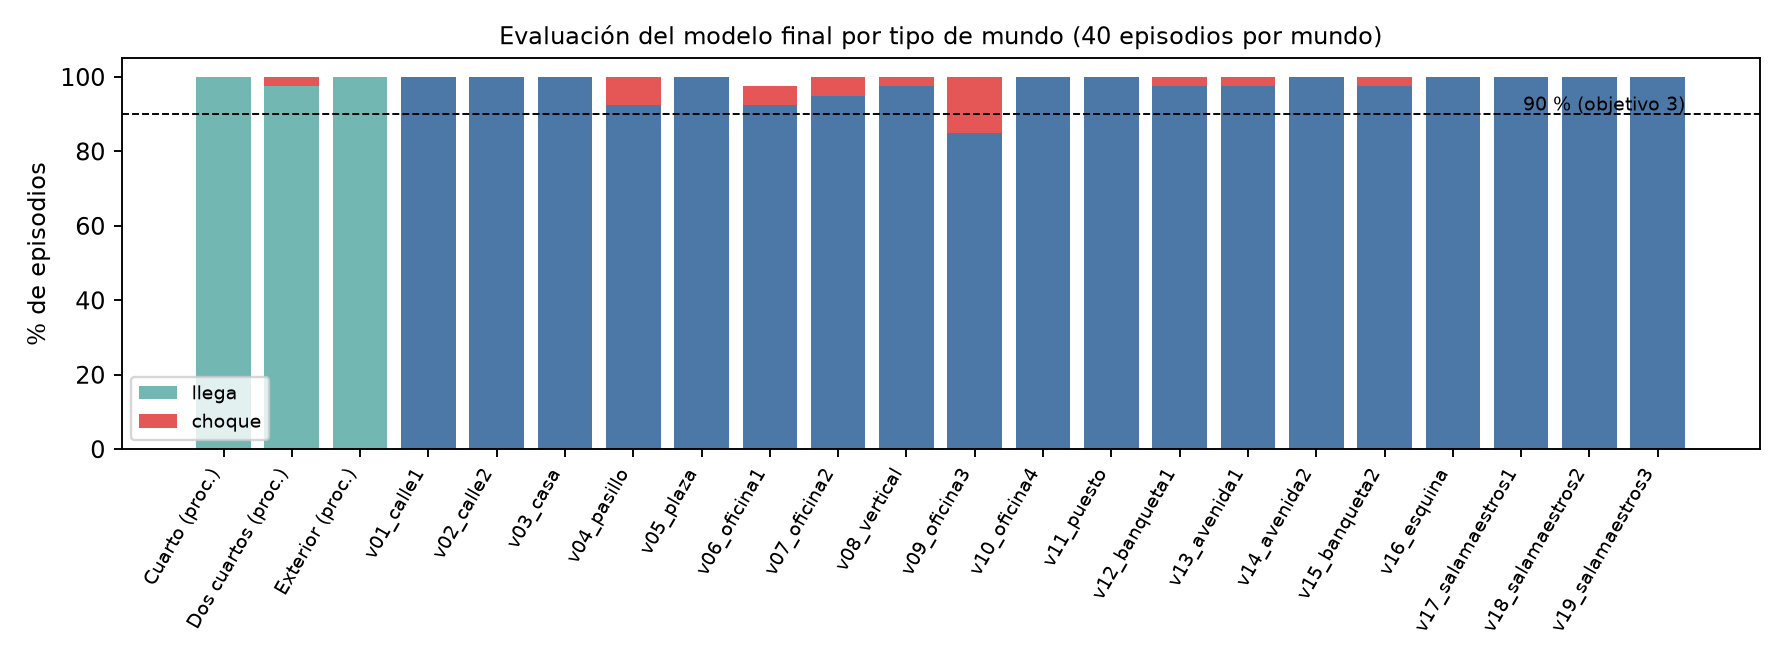
\includegraphics[width=\textwidth]{Capturas_TT2/nav/nav_eval_mundos.png}
    \caption{Porcentaje de episodios exitosos y con choque por mundo. En verde claro,
    mundos generados; en azul, mapas obtenidos de videos reales.}
    \label{fig:nav_eval}
\end{figure}

La Figura~\ref{fig:nav_episodios} muestra un episodio de cada tipo de mundo generado.
En el de dos cuartos, el agente se dirige primero hacia la puerta y cruza el vano; en
el exterior se aleja de las coladeras, aunque estas no aparecen en sus rayos.

\begin{figure}[H]
    \centering
    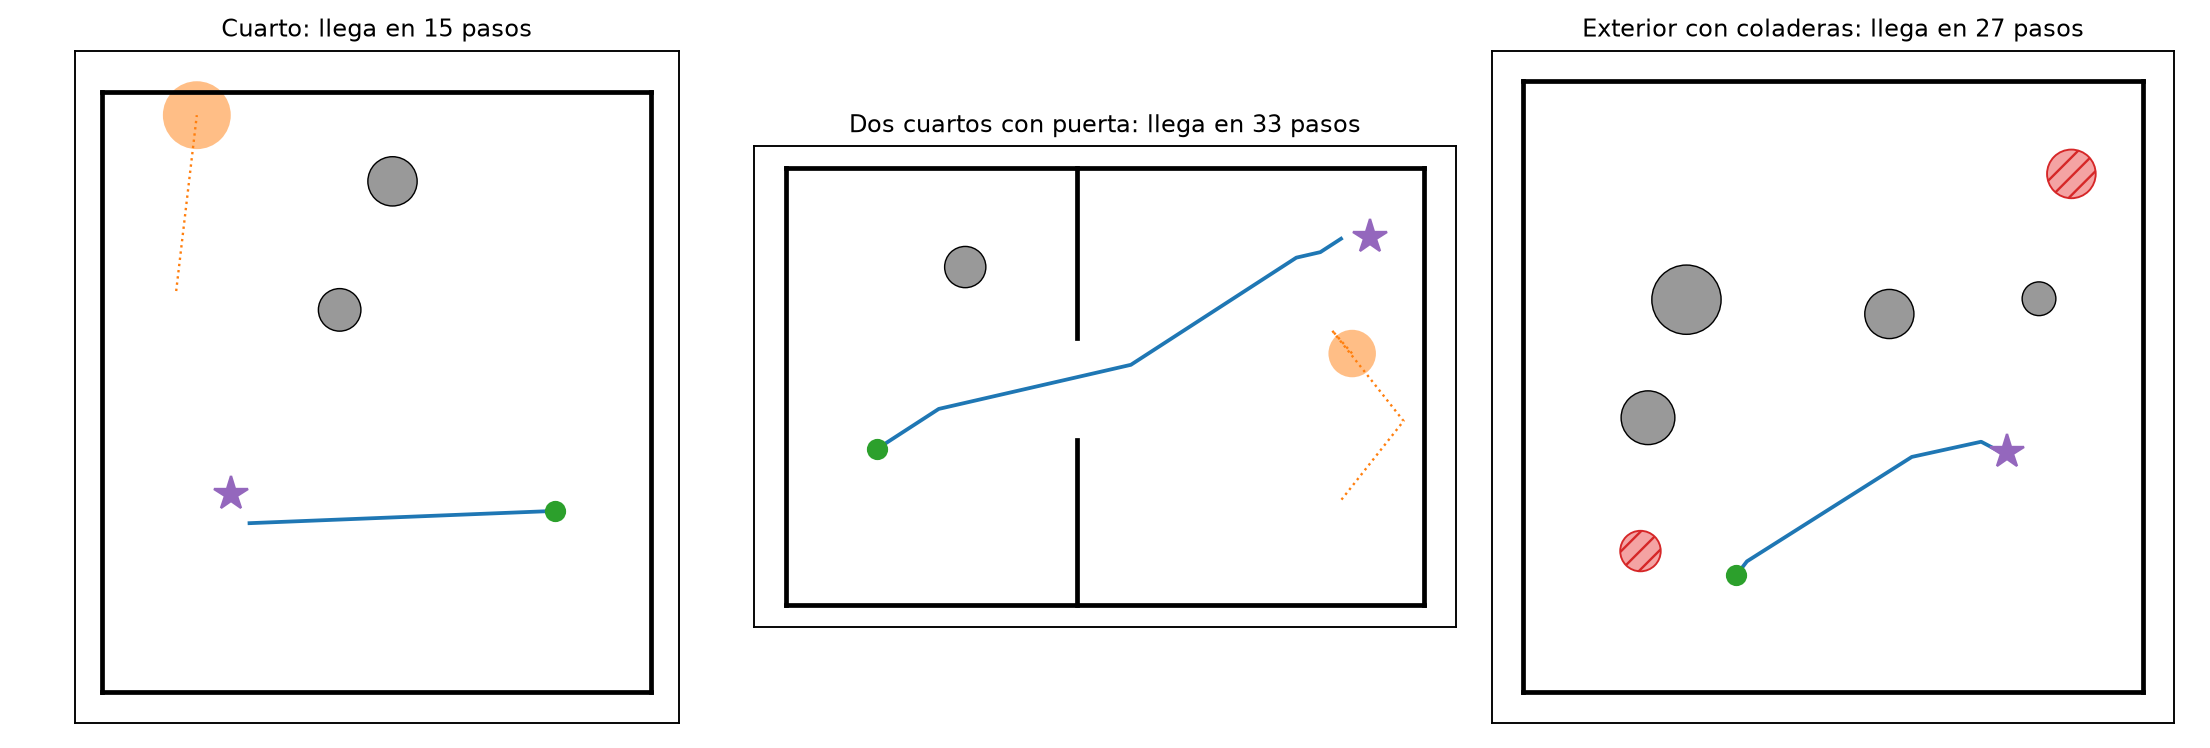
\includegraphics[width=\textwidth]{Capturas_TT2/nav/nav_episodios.png}
    \caption{Episodios del modelo final. Punto verde: inicio; estrella: meta; gris:
    obstáculos; rojo rayado: peligros de piso; naranja: persona en movimiento y su
    recorrido.}
    \label{fig:nav_episodios}
\end{figure}

\textbf{Sesiones completas en lazo cerrado.} La evaluación anterior mide al agente
dentro de su propio simulador. Para probar la cadena completa se ejecutaron sesiones
en el cuarto simulado con todos los módulos reales: sensores simulados, SLAM, mapa,
PLN, ejecutor y salida amigable. Un usuario virtual primero recorre el cuarto para
construir el mapa, después pide un destino por texto y a partir de ahí hace
exactamente lo que le indica el sistema. Se realizaron 20 sesiones (cinco semillas por
cuatro destinos) y en cada una se midió la distancia real entre el usuario y la
superficie del objeto en el momento en que el sistema anunció la llegada.

El sistema anunció la llegada en las 20 sesiones y el usuario nunca chocó, pero solo
en 7 quedó a menos de 1~m del objeto y en 12 a menos de 1.5~m. Al registrar qué
condición disparó cada llegada se encontró la causa (Tabla~\ref{tab:nav_lazo}): en 17
sesiones la llegada la decidió la regla de percepción, porque en un solo cuadro la
estimación monocular ubicó al objeto a menos de 1~m cuando en realidad estaba hasta a
2.5~m. Las tres llegadas decididas por la distancia en el mapa terminaron a menos de
0.8~m del objeto.

También se revisó si la validación con los ultrasónicos intervino en esas llegadas.
En 16 de las 17 el objeto quedaba fuera del cono angosto de los sensores (unos
$\pm 20^\circ$, mientras que la regla acepta objetos hasta $\pm 60^\circ$) o por
debajo del haz, así que el ultrasonido no pudo confirmar ni contradecir la distancia.
La única llegada con el objeto confirmado por ambos sensores terminó a 0.99~m, que es
una llegada correcta.

\begin{table}[H]
\centering
\caption{Sesiones en lazo cerrado según la condición que disparó la llegada}
\label{tab:nav_lazo}
\renewcommand{\arraystretch}{1.2}
\begin{tabular}{|p{5.2cm}|c|c|c|}
\hline
\textbf{Condición de llegada} & \textbf{Sesiones} & \textbf{Distancia real promedio}
& \textbf{A menos de 1~m} \\
\hline
Pose a menos de 0.6~m de la meta & 3 & 0.55~m & 3 \\
Objeto visto a menos de 1~m & 17 & 1.56~m & 4 \\
\hline
\textbf{Total} & \textbf{20} & & \textbf{7} \\
\hline
\end{tabular}
\end{table}

La regla de percepción resolvió un problema real, pero tal como está implementada es
demasiado sensible: basta un cuadro con un error monocular de 25 a 50\,\% para terminar
la sesión antes de tiempo. Exigir la condición durante varios cuadros seguidos, pedir
que el ultrasonido la confirme cuando el objeto está dentro de su cono, o combinarla
con la distancia en el mapa debería corregirlo.

La Figura~\ref{fig:nav_sesion} muestra una de estas sesiones. El usuario pidió
``llévame al sillón'' y en el paso 45 apareció una caja a 1.2~m delante de él. El
planificador cambió la ruta para pasar por debajo de la caja y el usuario siguió las
indicaciones hasta quedar a 0.75~m del sillón, donde la regla de percepción dio por
terminada la sesión. En corridas anteriores de la misma prueba se observó que el
primer plan después de la caja a veces todavía la atravesaba: el mapa necesita varios
ecos para convertir en ocupada una celda que ya había visto libre muchas veces
(Figura~\ref{fig:ray_logodds}).

\begin{figure}[H]
    \centering
    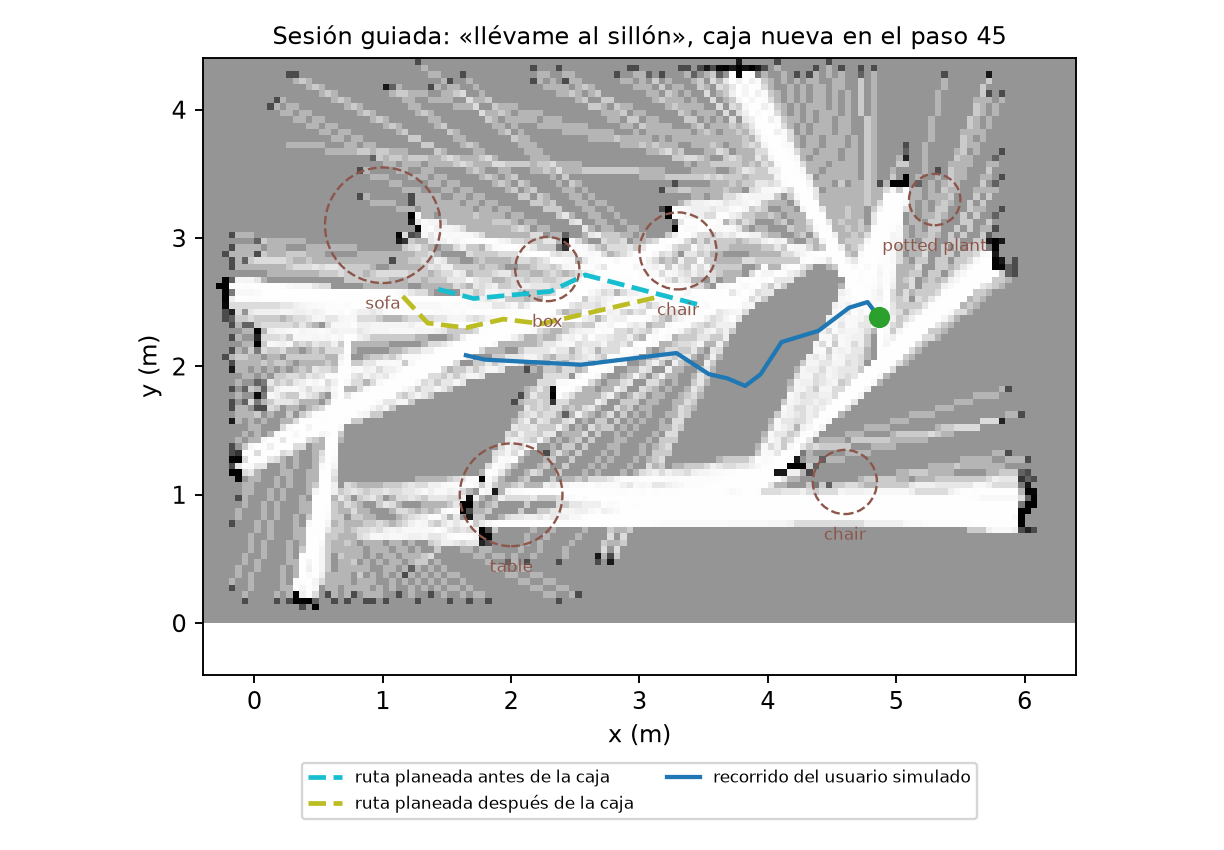
\includegraphics[width=0.82\textwidth]{Capturas_TT2/nav/nav_sesion_ok.png}
    \caption{Sesión en lazo cerrado con una caja que aparece en el camino. Las líneas
    discontinuas son las rutas que calculó el planificador antes y después de la
    caja.}
    \label{fig:nav_sesion}
\end{figure}

La Figura~\ref{fig:nav_vivo} muestra la vista de ruta de la interfaz de
\texttt{main\_nav\_lap.py} en dos momentos de esa sesión. En la segunda captura se
aprecia otro efecto del SLAM: el mapa ligero contiene \emph{landmarks} duplicados
(dos mesas y dos sillones en un cuarto que tiene uno de cada uno).

\begin{figure}[H]
    \centering
    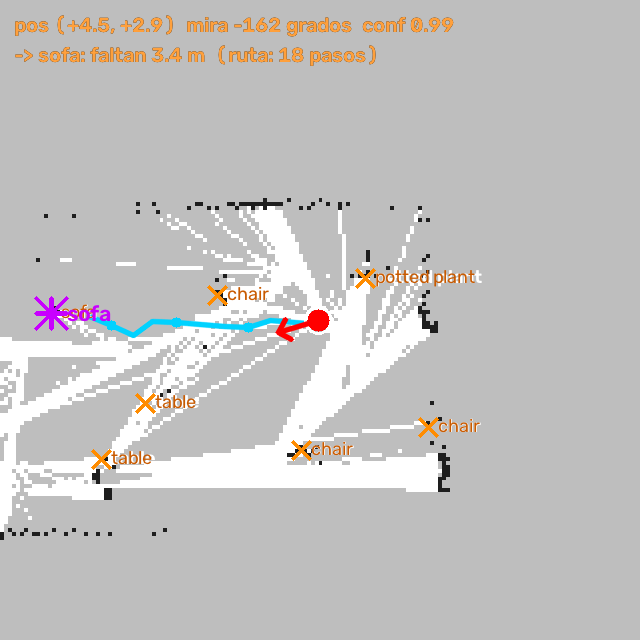
\includegraphics[width=0.48\textwidth]{Capturas_TT2/nav/nav_vivo_p10.png}
    \hfill
    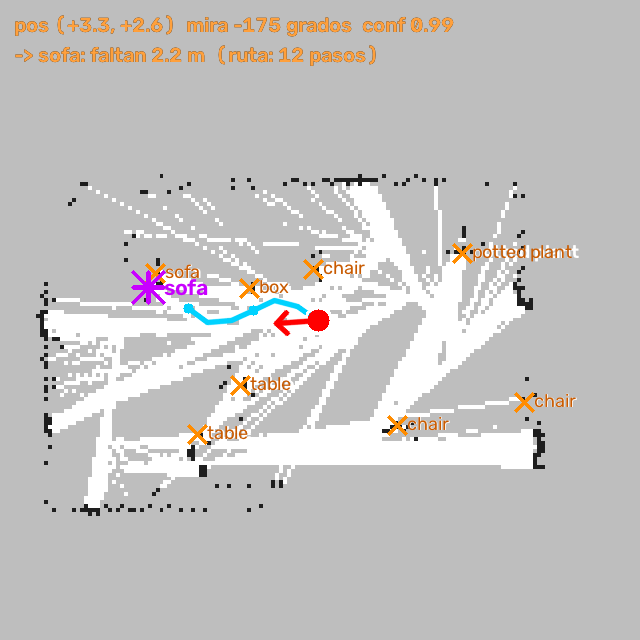
\includegraphics[width=0.48\textwidth]{Capturas_TT2/nav/nav_vivo_p52.png}
    \caption{Vista de ruta en vivo al inicio de la sesión (izquierda) y después de la
    caja (derecha). Cian: ruta planeada; estrella magenta: meta; cruces naranjas:
    \emph{landmarks}.}
    \label{fig:nav_vivo}
\end{figure}

Durante las sesiones se observaron otros dos detalles. Como en la simulación el
agente decide en cada ciclo, el sistema emitió en promedio una indicación cada 1.8
pasos, lo que en uso real sería demasiado; en el dispositivo el ritmo es de una
decisión por segundo y las indicaciones repetidas se agrupan. Además, el mensaje
amigable de llegada dice ``¡Llegamos! Ya estás en sofa'', porque usa la etiqueta en
inglés del \emph{landmark} en lugar del nombre que dijo el usuario.

\textbf{Costo computacional.} Construir la observación toma 0.64~ms, la inferencia
de la política 0.06~ms con Stable-Baselines3 y 0.01~ms con NumPy, y un plan completo
de ruta 7~ms. La navegación no limita la frecuencia del sistema.

\subsection{Limitaciones}

\begin{itemize}
    \item La llegada por percepción se dispara con un solo cuadro y termina sesiones
    antes de tiempo.
    \item Los resultados del 97.8\,\% corresponden al simulador del agente. En lazo
    cerrado con el SLAM y la percepción simulados, la llegada correcta a menos de 1~m
    bajó a 7 de 20 sesiones. Aún no se ha probado con una persona real.
    \item El riesgo por sector se calcula distinto en entrenamiento (a partir de la
    distancia a cualquier obstáculo) y en el sistema real (a partir de las
    detecciones de visión). Se intentó alinear el sistema real con la regla del
    entrenamiento y el desempeño empeoró, por lo que la corrección pendiente es del
    lado del entrenamiento.
    \item La solicitud de ruta alternativa reinicia el seguimiento del progreso, pero no
    obliga al agente a tomar un camino distinto.
    \item Los modelos de ruido del simulador se ajustaron sin los sensores físicos; al
    montar la IMU y los MB1232 habrá que medir el ruido real y reentrenar.
\end{itemize}
